\chapter{Swing-Up Design}\label{sec:swing-upDesign}
In this chapter four swing-up controllers are designed, all based on \cite{kjAastrom}. The pendulum is started at rest, $\theta = \pi$, with the angle convention specified in \autoref{fig:mechanicalDrawing}. The idea of the swing-up controller is to increase the mechanical energy in the system until it matches that of the desired end state, $\theta = 0$ and $\dot{\theta} = 0$, that is, the upright position at rest. The minimum energy in the system occurs at the starting position at rest, which is considered to be zero as mentioned in the \textit{Model} \autoref{sec:model}. So the target energy is $E_{\mathrm{eq}} = 2 m g l$, that is, the potential energy of the pendulum in the unstable equilibrium.

Consider the pendulum dynamics from \autoref{eq:energyDerivedDynamicEquation1}, where $J = m l^2$ is the pendulum inertia and frictions are assumed to be zero such that,
\begin{flalign}
&& J \ddot{\theta} - m l \cos \theta \ddot{x}_c - m g l \sin \theta  &= 0 \ \ \ , &  \unit{N \cdot m}   \label{eq:pendulumDynamics}
\end{flalign}
This equation captures the behavior of the pendulum corresponding to some acceleration $\ddot{x}_c$ at the pivot point. This acceleration is viewed as the control input for now. The force needed to achieve this acceleration is considered in the end of the design. It is further convenient to describe the energy of the pendulum with the coordinate frame fixed at its pivot point, see \autoref{fig:fixedCooredinateSystem}.
%
\begin{figure}[H]
  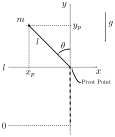
\includegraphics[width=.3\textwidth]{figures/fixedCooredinateSystem}
  \caption{The energy used in the swing-up controller is described using this convention, where the coordinate frame is fixed at the pivot point of the pendulum. The zero reference is placed as before s.t. all energies are positive.}
  \label{fig:fixedCooredinateSystem}
\end{figure}
%
From \autoref{fig:fixedCooredinateSystem}, the conversion from excessive to generalized coordinates is given by,
\begin{flalign}
&& x_p  &= -l \sin \theta   \ \ \ ,\ \ \ y_p = l(\cos \theta + 1)  \ \ \ ,\ \ \ \dot{x}_p = -l \cos \theta \dot{\theta}  \ \ \ ,\ \ \ \dot{y}_p = -l \sin \theta \dot{\theta}  \ \ \ . &&     \label{eq:cooredinateConvertFixed}
\end{flalign}
The mechanical energy in this coordinate frame is then,
\begin{flalign}
&& E_p &= m g y_p + \tfrac{1}{2} m \dot{x}_p^2 + \tfrac{1}{2} m \dot{y}_p^2  &  \unit{J}   \label{eq:pendulumEnergy1} \\
&& E_p &= m g l (\cos \theta +1) + \tfrac{1}{2} m (-l \cos \theta \dot{\theta})^2 + \tfrac{1}{2} m (-l \sin \theta \dot{\theta})^2  &  \unit{J}   \label{eq:pendulumEnergy2} \\
&& E_p &= m g l (\cos \theta +1) + \tfrac{1}{2} J (\cos^2 \theta  + \sin^2 \theta )\dot{\theta}^2  &  \unit{J}   \label{eq:pendulumEnergy3} \\
&& E_p &= \tfrac{1}{2} J \dot{\theta}^2 + m g l (\cos \theta +1) \ \ \ . &  \unit{J}   \label{eq:pendulumEnergy4}
\end{flalign}
The following sections explores different approaches of controlling the pendulum energy specified in \autoref{eq:pendulumEnergy4} to its desired reference.

\subsection{Energy Control}
A Lyapunov function candidate is proposed,
\begin{flalign}
&& V &= \tfrac{1}{2} E_\Delta ^2 \ \ \ ,  \hspace{5cm}  &&&  \label{eq:lyapunovCandidate} 
\end{flalign}
where $E_\Delta$ is the difference in energy in relation to the unstable equilibrium,
%
\begin{flalign}
&& E_\Delta &= E_p  - E_{\mathrm{eq}} &  \unit{J}   \label{eq:energyDelta1} \\
&& E_\Delta &= \tfrac{1}{2} J \dot{\theta}^2 + m g l (\cos \theta +1) - 2 m g l &  \unit{J}   \label{eq:energyDelta2} \\
&& E_\Delta &= \tfrac{1}{2} J \dot{\theta}^2 + m g l (\cos \theta -1)   \ \ \ .  & \unit{J} \label{eq:energyDelta3}
\end{flalign}
%
The derivative of $E_\Delta$ from \autoref{eq:energyDelta3} along the system \autoref{eq:pendulumDynamics} is found to,
\begin{flalign}
&& \dot{E}_\Delta &= J \dot{\theta} \ddot{\theta} - m g l \sin \theta \dot{\theta}  &&&   \label{eq:energyDeltaDerivative1} \\
&& \dot{E}_\Delta &= \dot{\theta} ( m l \cos \theta \ddot{x}_c + m g l \sin \theta )  - m g l \sin \theta \dot{\theta}    &&&   \label{eq:energyDeltaDerivative2} \\
&& \dot{E}_\Delta &=  m l \cos \theta \dot{\theta} \ddot{x}_c \ \ \ .   &&&   \label{eq:energyDeltaDerivative3}
\end{flalign}
%
The Lyapunov function candidate, \autoref{eq:lyapunovCandidate}, is continuously differentiable in the entire $\mathbb{R} ^2$. Its derivative is evaluated to find a stabilizing controller,
%
\begin{flalign}
&& \dot{V} &= E_\Delta \dot{E}_\Delta   \hspace{3cm}  &&&  \label{eq:lyapunovDerivative1}  \\
&& \dot{V} &= E_\Delta m l \cos \theta \dot{\theta} \ddot{x}_c  \leq 0  \ \ \ .  \hspace{3cm}  &&&  \label{eq:lyapunovDerivative2} 
\end{flalign}
%
The acceleration, $\ddot{x}_c$, is then designed to satisfy the stability criterion in \autoref{eq:lyapunovDerivative2},
\begin{flalign}
&& \dot{V} &= m l E_\Delta \cos \theta \dot{\theta} (-E_\Delta \cos \theta \dot{\theta})     \hspace{2cm}  &&&  \label{eq:lyapunovDerivativeControlled1} \\
&& \dot{V} &= -m l (E_\Delta \cos \theta \dot{\theta})^2  \leq 0  \ \ \ ,  \hspace{2cm}  &&&  \label{eq:lyapunovDerivativeControlled2} 
\end{flalign}
further a tuning parameter, $k>0$, is introduced such that the control law for the acceleration of the pivot point is,
\begin{flalign}
&& \ddot{x}_c &= -k E_\Delta \cos \theta \dot{\theta}  \ \ \ .  \hspace{4cm}  &&&  \label{eq:accControlLaw} 
\end{flalign}
If this control law is started at zero angular velocity, $\dot{\theta} = 0$, in a stable equilibrium, the computed control is maintained at zero and the pendulum never swings up. So for this control law to work, the pendulum must be started slightly away from a stable equilibrium. The control is also zero when $\cos\theta = 0$, however, when this occurs the system is not in a stable equilibrium and the zero value of $\ddot{x}_c$ is therefore not maintained in these cases.

An extra step is needed to apply this control strategy. So far the control output is an acceleration, $\ddot{x}_c$, at the pivot point. It is possible to input the desired acceleration, $\ddot{x}_c$, into the second dynamic equation, \autoref{eq:energyDerivedDynamicEquation1}, and solve for the force needed to achieve this acceleration,
%
\begin{flalign}
  && u &=  ( M + m )\ddot{x}_c + m l \sin x_1 x_3^2 - m l \cos x_1 \dot{x}_3  \ \ \ , &   \unit{N}
  \label{eq:forceDynamics}
\end{flalign}
%
where the cart friction coefficients are set to zero again.\\
To calculate the force from this expression, \autoref{eq:forceDynamics}, it is also necessary to know the angular acceleration of the pendulum, $\dot{x}_3$, which can be solved for in the system dynamics, \autoref{eq:nonlinearStateSpace}, inserting known states and control input applied in the previous step,
%
\begin{flalign}
  &&
    \begin{bmatrix}
      \dot{x}_3  \\
      \dot{x}_4
    \end{bmatrix}
    &=
    \begin{bmatrix}
      m l^2           & -m l \cos x_1  \\
      -m l \cos x_1   & M + m
    \end{bmatrix}^{-1}
    \begin{bmatrix}
      - b_{p,v} x_3 - \tanh(\text{k}_\text{tanh}x_3) b_{p,c} + m g l \sin x_1 \\
      u_{last} - m l \sin x_1 x_3^2
    \end{bmatrix}
     \ \ \ ,  &&
  \label{eq:nonlinearStateSpaceQdotDot}
\end{flalign}
%
where $u_{last}$ is the force applied in the previous step.\\
From \autoref{eq:nonlinearStateSpaceQdotDot} the approximated angular acceleration is then,
\begin{flalign}
  && \dot{x}_3 &= \frac{ ( M + m )(- b_{p,v} x_3 - \tanh(\text{k}_\text{tanh}x_3) b_{p,c} + m g l \sin x_1) }{ l^2 m ( M + m - m \cos^2x_1 ) }
                    + \frac{ \cos x_1 (u_{last} - m l \sin x_1 x_3^2) }{ l ( M + m - m \cos x_1^2 ) }
  \ \ \ .  &&
  \label{eq:thetaDotDotApprox}
\end{flalign}
%
Inserting \autoref{eq:thetaDotDotApprox} into \autoref{eq:forceDynamics} results in the control input, $u$, necessary to achieve the desired acceleration, $\ddot{x}_c$, at the pivot point. This method is used for all four swing-up controllers, so to avoid excessive notation the proceeding energy control laws are derived with $\ddot{x}_c$ as the control parameter.

All simulations are performed using the nonlinear state space representation in \autoref{eq:nonlinearStateSpace} and the matlab ODE45 solver with relative tolerance of \SI{1e-7}{}. Initializing the angle, $\theta$, at $\pi-0.1$ to avoid zero control output as discussed, the energy difference struggles to reach its reference at zero, see \autoref{fig:Edelta_1_noConX}. The pendulum friction and cart inertia are included in the calculation of the force needed to obtain the desired acceleration. This, however, is not concerned with what is needed to obtain the required energy. So the offset seen in \autoref{fig:Edelta_1_noConX} is caused by the control law, \autoref{eq:accControlLaw}, asking for insufficient acceleration.
%
\begin{figure}[H]
  \hspace{-10pt}
  \captionbox
  {
    Simulation of the first energy control method. The energy error struggles to maintain zero value, due to pendulum friction and cart inertia exchanging energy with the pendulum.
    \label{fig:Edelta_1_noConX}
  }
  {
    \hspace{-1cm}
    \includegraphics[width=.46\textwidth]{figures/Edelta_1_noConX}
  }
  \hspace{20pt}
  \captionbox 
  {
    This phase portrait shows the attempt to reach the heteroclinic orbit. It falls short due to the insufficient acceleration asked by the control law.
    \label{fig:phase_1_noConX}
  }
  {
    \hspace{-1cm}
    \includegraphics[width=.46\textwidth]{figures/phase_1_noConX}
  }  
\end{figure}
%
The pendulum also falls short of reaching the heteroclinic orbit, see \autoref{fig:phase_1_noConX}.
Further, since the energy of the pendulum is not affected by the position or velocity of the cart, this control law, \autoref{eq:accControlLaw}, is not concerned with controlling these. This becomes a problem in the physical setup as it has a rail length of \SI{0.89}{m}, see \autoref{table:systemParameters}. A traced animation is used to demonstrate this problem in \autoref{fig:ani_1_noConX}.
\begin{figure}[H]
  \includegraphics[width=.7\textwidth]{figures/ani_1_noConX}
  \caption{The cart drifts beyond the bounds of the physical system. This might not be a problem if the catch controller catches the pendulum in first try, but there is no guarantee of this being the case.}
  \label{fig:ani_1_noConX}
\end{figure}
%
An other issue is the actuation which is limited in the real system by the maximum allowed continuous current, see \autoref{table:systemParameters}. By tuning the parameter $k$ in \autoref{eq:accControlLaw}, better performance can be obtained, however at the cost of excessive actuation.
%
\begin{figure}[H]
  \includegraphics[width=.52\textwidth]{figures/ia_1_noConX}
  \caption{The motor current has high peaks in the beginning which likely exceeds the capabilities of the motor. The controller is tuned such that the RMS value of the current does not exceed the maximum continuous current requirement of the motor for a sustained period of time.}
  \label{fig:ia_1_noConX}
\end{figure}
%
For these graphs $k=1.3$ to keep the motor current at acceptable levels. The motor current is shown in \autoref{fig:ia_1_noConX} where the rolling RMS of $i_a$ is used to approximate the continuous current load on the motor.

%\begin{figure}[H]
%  \includegraphics[width=.6\textwidth]{figures/x_1_noConX}
%  \caption{x1noConX}
%  \label{fig:x_1_noConX}
%\end{figure}
%\begin{figure}[H]
%  \includegraphics[width=.6\textwidth]{figures/xDot_1_noConX}
%  \caption{xDot1noConX}
%  \label{fig:xDot_1_noConX}
%\end{figure}
%\begin{figure}[H]
%  \includegraphics[width=.6\textwidth]{figures/xDotDot_1_noConX}
%  \caption{xDotDot1noConX}
%  \label{fig:xDotDot_1_noConX}
%\end{figure}
%\begin{figure}[H]
%  \includegraphics[width=.6\textwidth]{figures/theta_1_noConX}
%  \caption{theta1noConX}
%  \label{fig:theta_1_noConX}
%\end{figure}
%\begin{figure}[H]
%  \includegraphics[width=.6\textwidth]{figures/thetaDot_1_noConX}
%  \caption{thetaDot1noConX}
%  \label{fig:thetaDot_1_noConX}
%\end{figure}
%\begin{figure}[H]
%  \includegraphics[width=.6\textwidth]{figures/thetaDotDot_1_noConX}
%  \caption{thetaDotDot1noConX}
%  \label{fig:thetaDotDot_1_noConX}
%\end{figure}


\subsection{Sign-Based Energy Control}
There are other ways to satisfy \autoref{eq:lyapunovDerivativeControlled2} than the control law suggested in \autoref{eq:accControlLaw}. To achieve maximal actuation a sign-function can be used to determine the direction of actuation along with a gain $k$ to adjust for the limits of the actuator,
\begin{flalign}
  && \ddot{x}_c &= k\ \mathrm{sgn}(-E_\Delta \cos \theta \dot{\theta})  \ \ \ ,  \hspace{4cm}  &&&  \label{eq:accControlLaw2} 
\end{flalign}
where sgn is redefined to be one if it outputs zero, to avoid no actuation when starting at stable equilibrium. The gain is tuned to $k = 2.7$ in the following simulation. Looking at the energy in \autoref{fig:Edelta_2_noConX} this strategy seems to work really well. From the phase plot in \autoref{fig:phase_2_noConX} it is evident that a near perfect heteroclinic orbit is reached.
\begin{figure}[H]
  \hspace{-10pt}
  \captionbox
  {
    Edelta2noConX
    \label{fig:Edelta_2_noConX}
  }
  {
    \hspace{-1cm}
    \includegraphics[width=.46\textwidth]{figures/Edelta_2_noConX}
  }
  \hspace{20pt}
  \captionbox 
  {
    phase2noConX
    \label{fig:phase_2_noConX}
  }
  {
    \hspace{-1cm}
    \includegraphics[width=.46\textwidth]{figures/phase_2_noConX}
  }  
\end{figure}
%
In \autoref{fig:ani_2_noConX} however, while the angle reaches the equilibrium as closely as possible without overshooting, this control law, as with the previous, does not account for position of the cart.
%
\begin{figure}[H]
  \includegraphics[width=1\textwidth]{figures/ani_2_noConX}
  \caption{ani2noConX}
  \label{fig:ani_2_noConX}
\end{figure}
%
However, the bigger problem with this control law is obvious from \autoref{fig:ia_2_noConX}, where excessive switching shows on the control output. This actuation behavior is not feasible in a real system and attempted implementation will cause chattering resulting in unwanted behavior and wear of the motor.
%
\begin{figure}[H]
  \includegraphics[width=.52\textwidth]{figures/ia_2_noConX}
  \caption{ia2noConX}
  \label{fig:ia_2_noConX}
\end{figure}
%
%\begin{figure}[H]
%  \includegraphics[width=.6\textwidth]{figures/x_2_noConX}
%  \caption{x2noConX}
%  \label{fig:x_2_noConX}
%\end{figure}
%\begin{figure}[H]
%  \includegraphics[width=.6\textwidth]{figures/xDot_2_noConX}
%  \caption{xDot2noConX}
%  \label{fig:xDot_2_noConX}
%\end{figure}
%\begin{figure}[H]
%  \includegraphics[width=.6\textwidth]{figures/xDotDot_2_noConX}
%  \caption{xDotDot2noConX}
%  \label{fig:xDotDot_2_noConX}
%\end{figure}
%\begin{figure}[H]
%  \includegraphics[width=.6\textwidth]{figures/theta_2_noConX}
%  \caption{theta2noConX}
%  \label{fig:theta_2_noConX}
%\end{figure}
%\begin{figure}[H]
%  \includegraphics[width=.6\textwidth]{figures/thetaDot_2_noConX}
%  \caption{thetaDot2noConX}
%  \label{fig:thetaDot_2_noConX}
%\end{figure}
%\begin{figure}[H]
%  \includegraphics[width=.6\textwidth]{figures/thetaDotDot_2_noConX}
%  \caption{thetaDotDot2noConX}
%  \label{fig:thetaDotDot_2_noConX}
%\end{figure}
%
%
%
It is possible to implement a less aggressive version of this idea by using a saturation function to approximate the sign function around zero,
\begin{flalign}
  && \ddot{x}_c &= k\ \mathrm{sat}(-\tfrac{1}{\varepsilon}E_\Delta \cos \theta \dot{\theta})  \ \ \ ,  \hspace{4cm}  &&&  \label{eq:accControlLaw2_2} 
\end{flalign}
where $\varepsilon$ decides the slope of the saturation function around zero,
\begin{flalign}
  &&\text{sat}\left( \frac{c}{\varepsilon} \right) &=
  \begin{cases}
    \ \ \frac{c}{\varepsilon}                             &, \ \ \ \ \mathrm{if} \ | \frac{c}{\varepsilon} | \leq 1 \\
    \ \ \mathrm{sgn}\left( \frac{c}{\varepsilon} \right)  &, \ \ \ \ \mathrm{if} \ | \frac{c}{\varepsilon} |  >   1 \ \ \ ,
  \end{cases} &&& 
  \label{eq:satuationFunction1}
\end{flalign}
where $c$ is an input to the sat-function.
In the simulation $k = 2.7$ as before and $\varepsilon = 0.01$ to avoid excessive switching while maintaining a relatively close approximation of the sign-function. This control strategy achieves the energy reference in about three seconds, \autoref{fig:Edelta_3_noConX}, as is the case of the sign strategy, \autoref{fig:Edelta_2_noConX}. Further, from \autoref{fig:phase_3_noConX}, the system still reaches a near perfect heteroclinic orbit.
%
\begin{figure}[H]
  \hspace{-10pt}
  \captionbox
  {
    Edelta3noConX
    \label{fig:Edelta_3_noConX}
  }
  {
    \hspace{-1cm}
    \includegraphics[width=.46\textwidth]{figures/Edelta_3_noConX}
  }
  \hspace{20pt}
  \captionbox 
  {
    phase3noConX
    \label{fig:phase_3_noConX}
  }
  {
    \hspace{-1cm}
    \includegraphics[width=.46\textwidth]{figures/phase_3_noConX}
  }  
\end{figure}
%
The cart still drifts as expected, see \autoref{fig:ani_3_noConX}.
%
\begin{figure}[H]
  \includegraphics[width=.7\textwidth]{figures/ani_3_noConX}
  \caption{ani3noConX}
  \label{fig:ani_3_noConX}
\end{figure}
%
The excessive switching on the control output is successfully avoided, see \autoref{fig:ia_3_noConX}, resulting in a much more realistic control signal compared to that in \autoref{fig:ia_2_noConX}.
%
\begin{figure}[H]
  \includegraphics[width=.52\textwidth]{figures/ia_3_noConX}
  \caption{ia3noConX}
  \label{fig:ia_3_noConX}
\end{figure}
%
%
%\begin{figure}[H]
%  \includegraphics[width=.6\textwidth]{figures/x_3_noConX}
%  \caption{x3noConX}
%  \label{fig:x_3_noConX}
%\end{figure}
%\begin{figure}[H]
%  \includegraphics[width=.6\textwidth]{figures/xDot_3_noConX}
%  \caption{xDot3noConX}
%  \label{fig:xDot_3_noConX}
%\end{figure}
%\begin{figure}[H]
%  \includegraphics[width=.6\textwidth]{figures/xDotDot_3_noConX}
%  \caption{xDotDot3noConX}
%  \label{fig:xDotDot_3_noConX}
%\end{figure}
%\begin{figure}[H]
%  \includegraphics[width=.6\textwidth]{figures/theta_3_noConX}
%  \caption{theta3noConX}
%  \label{fig:theta_3_noConX}
%\end{figure}
%\begin{figure}[H]
%  \includegraphics[width=.6\textwidth]{figures/thetaDot_3_noConX}
%  \caption{thetaDot3noConX}
%  \label{fig:thetaDot_3_noConX}
%\end{figure}
%\begin{figure}[H]
%  \includegraphics[width=.6\textwidth]{figures/thetaDotDot_3_noConX}
%  \caption{thetaDotDot3noConX}
%  \label{fig:thetaDotDot_3_noConX}
%\end{figure}


\subsection{Sat-Based Energy Control}
An other strategy to avoid the excessive switching of the sign-controller is presented here,
\begin{flalign}
  && \ddot{x}_c &= \mathrm{sat}(-k E_\Delta \mathrm{sgn}(\cos \theta \dot{\theta}))  \ \ \ ,  \hspace{4cm}  &&&  \label{eq:accControlLaw3} 
\end{flalign}
where the saturation function is saturates at the maximum/minimum allowed acceleration. The known limitation is $i_{max} = 4.58$ as stated in \autoref{table:systemParameters}, from which the maximum control, $u$, can be calculated,
\begin{flalign}
  && u_{max} &=  \frac{k_{\tau}}{r} \ \ \ ,  \hspace{4cm}  &&&  \label{eq:maxU} 
\end{flalign}
and finally by disregarding the pendulum behavior and cart friction from the dynamics in \autoref{eq:energyDerivedDynamicEquation1},
\begin{flalign}
  && a_{max} &= \frac{u_{max}}{M+m} \ \ \ .  \hspace{4cm}  &&&  \label{eq:maxAcc} 
\end{flalign}
As this is a crude estimation $0.2$ is subtracted from the estimated $a_{max}$ in following simulations to stay within the actuation limits. The saturation function is then,
\begin{flalign}
  &&\text{sat}(c) &=
  \begin{cases}
    \ \ c                          &, \ \ \ \ \mathrm{if} \ | c | \leq a_{max} \\
    \ \ \mathrm{sgn}( c )\ a_{max}  &, \ \ \ \ \mathrm{if} \ | c |  >   a_{max} \ \ \ ,
  \end{cases} &&& 
  \label{eq:satuationFunction2}
\end{flalign}
where $c$ is the input to the sat-function. Again, the sign function is redefined to one in cases where it obtains a zero value.
Choice of $k$ in \autoref{eq:accControlLaw3} decides how aggressive the controller should be. Larger values of $k$ drives the control into saturation faster thus actuating more like the sign-based controller in \autoref{eq:accControlLaw2}. At lower values of $k$ the operation will not reach saturation as fast thus behaving more like the first energy based controller in \autoref{eq:accControlLaw}. For an effective swing up behavior $k=200$ is used putting the control closer to that of the sign-based controller, which makes sense as this was the theoretically ideal option.\\
The performance in \autoref{fig:Edelta_4_noConX} is similar to that in \autoref{fig:Edelta_3_noConX} and again the system reaches a near perfect heteroclinic orbit in \autoref{fig:phase_4_noConX}.
%
\begin{figure}[H]
  \hspace{-10pt}
  \captionbox
  {
    Edelta4noConX
    \label{fig:Edelta_4_noConX}
  }
  {
    \hspace{-1cm}
    \includegraphics[width=.46\textwidth]{figures/Edelta_4_noConX}
  }
  \hspace{20pt}
  \captionbox 
  {
    phase4noConX
    \label{fig:phase_4_noConX}
  }
  {
    \hspace{-1cm}
    \includegraphics[width=.46\textwidth]{figures/phase_4_noConX}
  }  
\end{figure}
%
The overall behavior also closely mimics that of \autoref{fig:ani_3_noConX} as seen in \autoref{fig:ani_4_noConX}.
\begin{figure}[H]
  \includegraphics[width=.7\textwidth]{figures/ani_4_noConX}
  \caption{ani4noConX}
  \label{fig:ani_4_noConX}
\end{figure}
%
There is however a slight difference in the control signal. In \autoref{fig:ia_4_noConX} less switching occurs compared to \autoref{fig:ia_3_noConX}. 
\begin{figure}[H]
  \includegraphics[width=.52\textwidth]{figures/ia_4_noConX}
  \caption{ia4noConX}
  \label{fig:ia_4_noConX}
\end{figure}
%
Two of the four investigated controller designs are deemed good candidates, namely \autoref{eq:accControlLaw2_2} and \autopageref{eq:accControlLaw3}. The problem of controlling the cart position still remains. The performances of the two control law candidates are compared as they are subjected to the disturbance caused by added control on the cart position and velocity.
%
%
%\begin{figure}[H]
%  \includegraphics[width=.6\textwidth]{figures/x_4_noConX}
%  \caption{x4noConX}
%  \label{fig:x_4_noConX}
%\end{figure}
%\begin{figure}[H]
%  \includegraphics[width=.6\textwidth]{figures/xDot_4_noConX}
%  \caption{xDot4noConX}
%  \label{fig:xDot_4_noConX}
%\end{figure}
%\begin{figure}[H]
%  \includegraphics[width=.6\textwidth]{figures/xDotDot_4_noConX}
%  \caption{xDotDot4noConX}
%  \label{fig:xDotDot_4_noConX}
%\end{figure}
%\begin{figure}[H]
%  \includegraphics[width=.6\textwidth]{figures/theta_4_noConX}
%  \caption{theta4noConX}
%  \label{fig:theta_4_noConX}
%\end{figure}
%\begin{figure}[H]
%  \includegraphics[width=.6\textwidth]{figures/thetaDot_4_noConX}
%  \caption{thetaDot4noConX}
%  \label{fig:thetaDot_4_noConX}
%\end{figure}
%\begin{figure}[H]
%  \includegraphics[width=.6\textwidth]{figures/thetaDotDot_4_noConX}
%  \caption{thetaDotDot4noConX}
%  \label{fig:thetaDotDot_4_noConX}
%\end{figure}

\subsection{Cart Position and Velocity Control}
To solve the cart drifting problem along $x$ a linear controller is designed and added to the control law,
\begin{flalign}
  && \ddot{x}_c &= \psi(x_1,x_3) + v(x_2,x_4) \ \ \ ,  \hspace{4cm}  &&&  \label{eq:combiControl} 
\end{flalign}
where $\psi(x_1,x_3)$ is the energy controller and $v(x_2,x_4)$ is the linear controller. While these two controllers depend on different states, they still influence and act as unmodeled disturbances to each other. The position and velocity control, $v(x_2,x_4)$, adds and subtracts energy and therefore could cause the energy controller, $\psi(x_1,x_3)$, to overshoot. One solution to this potential problem could be to slightly lower the energy reference. However, swing-up is often designed with a slightly higher energy reference such that the catch controller has some entry velocity at the unstable equilibrium.\\
With these considerations in mind, the design of $v(x_2,x_4)$ is proceeded. Considering the cart without friction and assuming that any influence of the pendulum and the energy control to be unmodeled disturbances of the system. This reduces the system to the mechanical drawing seen in \autoref{fig:mechanicalDrawingSimple}.
%
\begin{figure}[H]
  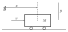
\includegraphics[width=.35\textwidth]{figures/mechanicalDrawingSimple}
  \caption{mechanicalDrawingSimple}
  \label{fig:mechanicalDrawingSimple}
\end{figure}
%
The dynamics are then,
\begin{flalign}
  && M \ddot{x} &=  v \ \ \ ,  \hspace{4cm}  &&&  \label{eq:simpleDynamics} 
\end{flalign}
and selecting new states $ [\ x_1\ \ x_2\ ]^\mathrm{T} = [\ x\ \ \dot{x}\ ]^\mathrm{T} $, the linear state space is,
\begin{flalign}
  &&
  \begin{bmatrix}
    \dot{x_1} \\
    \dot{x_2}
  \end{bmatrix}
  &=
  \underbrace{
    \begin{bmatrix}
      0 & 1 \\
      0 & 0
    \end{bmatrix}
  }_{A}
  \begin{bmatrix}
    x_1 \\
    x_2
  \end{bmatrix}
  +
  \underbrace{
    \begin{bmatrix}
      0 \\
      \tfrac{1}{M}
    \end{bmatrix}
  }_{B}
  v
  \label{eq:simpleLinearStateSpace} \ \ \ . &&&
\end{flalign}
%
The closed loop poles are placed in $p = [\ -1\ -2 \ ] $ using matlab \textit{place()}-command to obtain linear feedback gains, $\vec{k_1} = [\ 10.5460\ \ 15.8190\ ]$, resulting in the controller,
\begin{flalign}
  && v &= -\vec{k_1} \vec{x} \ \ \ ,  \hspace{4cm}  &&&  \label{eq:linearFeedbackSimple} 
\end{flalign}
where $\vec{x} = [\ x\ \ \dot{x}\ ]^\mathrm{T}$, such that,
\begin{flalign}
  && v(x_2,x_4) &= -\vec{k_1}  [\ x_2\ \ x_4\ ]^\mathrm{T} \ \ \ ,  \hspace{4cm}  &&&  \label{eq:linearFeedbackSimple2} 
\end{flalign}
in therms of the full system. This control is added to both of the considered energy control approaches and simulations are run without changing any previously designed gains.
\autoref{fig:Edelta_3_conX} shows the energy difference in the approximated sign approach while \autoref{fig:Edelta_4_conX} shows the sat-based approach. The approximated sign control approaches the reference slightly faster, however both reaches the reference at the same time.
%
\begin{figure}[H]
  \hspace{-10pt}
  \captionbox
  {
    Edelta3ConX
    \label{fig:Edelta_3_conX}
  }
  {
    \hspace{-1cm}
    \includegraphics[width=.46\textwidth]{figures/Edelta_3_conX}
  }
  \hspace{20pt}
  \captionbox 
  {
    Edelta4ConX
    \label{fig:Edelta_4_conX}
  }
  {
    \hspace{-1cm}
    \includegraphics[width=.46\textwidth]{figures/Edelta_4_conX}
  }  
\end{figure}
%
In the phase portraits, see \autoref{fig:phase_3_conX} and \ref{fig:phase_4_conX}, both control strategies reaches the heteroclinic orbit. However the approximated sign approach comes slightly closer in the swing preceding the orbit. If it is close enough that a catch controller could catch it, one swing could be saved.
\begin{figure}[H]
  \hspace{-10pt}
  \captionbox
  {
    phase3ConX
    \label{fig:phase_3_conX}
  }
  {
    \hspace{-1cm}
    \includegraphics[width=.46\textwidth]{figures/phase_3_conX}
  }
  \hspace{20pt}
  \captionbox 
  {
    phase4ConX
    \label{fig:phase_4_conX}
  }
  {
    \hspace{-1cm}
    \includegraphics[width=.46\textwidth]{figures/phase_4_conX}
  }  
\end{figure}
%
This fact is also seen in \autoref{fig:ani_3_conX} where the trace of the swing preceding the heteroclinic orbit reaches higher than in \autoref{fig:ani_4_conX}. These figures also show that the linear control of the cart position and velocity successfully keeps the system within the accessible operating region of the real system.
%
\begin{figure}[H]
  \hspace{-10pt}
  \captionbox
  {
    ani3ConX
    \label{fig:ani_3_conX}
  }
  {
    \hspace{-1cm}
    \includegraphics[width=.46\textwidth]{figures/ani_3_conX}
  }
  \hspace{20pt}
  \captionbox 
  {
    ani4ConX
    \label{fig:ani_4_conX}
  }
  {
    \hspace{-1cm}
    \includegraphics[width=.46\textwidth]{figures/ani_4_conX}
  }  
\end{figure}
%
\autoref{fig:ia_3_conX} shows the actuation of the approximated sign approach, where the added linear control has caused less switching compared to \autoref{fig:ia_3_noConX}. In fact, both control strategies show very similar output when comparing to \autoref{fig:ia_4_conX}. In both cases the RMS is lower than before the added linear controller. This could be tuned more tightly, but is left as a margin for now, with the possibility of further tuning during implementation.
%
\begin{figure}[H]
  \hspace{-10pt}
  \captionbox
  {
    ia3ConX
    \label{fig:ia_3_conX}
  }
  {
    \hspace{-1cm}
    \includegraphics[width=.46\textwidth]{figures/ia_3_conX}
  }
  \hspace{20pt}
  \captionbox 
  {
    ia4ConX
    \label{fig:ia_4_conX}
  }
  {
    \hspace{-1cm}
    \includegraphics[width=.46\textwidth]{figures/ia_4_conX}
  }  
\end{figure}
%
\autoref{fig:x_3_conX} and \ref{fig:x_4_conX} show the position approaching zero as the energy control settles, which is ideal, as it means the energy controllers still have room to operate without fighting the linear feedback controller too much. Similarly, the oscillations around zero are necessary for the energy controller to keep its reference.
%
\begin{figure}[H]
  \hspace{-10pt}
  \captionbox
  {
    x3ConX
    \label{fig:x_3_conX}
  }
  {
    \hspace{-1cm}
    \includegraphics[width=.4\textwidth]{figures/x_3_conX}
  }
  \hspace{20pt}
  \captionbox 
  {
    x4ConX
    \label{fig:x_4_conX}
  }
  {
    \hspace{-1cm}
    \includegraphics[width=.4\textwidth]{figures/x_4_conX}
  }  
\end{figure}
The same is seen for the velocity in \autoref{fig:xDot_3_conX} and \ref{fig:xDot_4_conX}. These four graphs are simulated over longer time to show that the linear controller reaches its reference.
\begin{figure}[H]
  \hspace{-10pt}
  \captionbox
  {
    xDot3ConX
    \label{fig:xDot_3_conX}
  }
  {
    \hspace{-1cm}
    \includegraphics[width=.4\textwidth]{figures/xDot_3_conX}
  }
  \hspace{20pt}
  \captionbox 
  {
    xDot4ConX
    \label{fig:xDot_4_conX}
  }
  {
    \hspace{-1cm}
    \includegraphics[width=.4\textwidth]{figures/xDot_4_conX}
  }  
\end{figure}







%
%
%
%\begin{figure}[H]
%  \includegraphics[width=.6\textwidth]{figures/xDotDot_3_conX}
%  \caption{xDotDot3ConX}
%  \label{fig:xDotDot_3_conX}
%\end{figure}
%\begin{figure}[H]
%  \includegraphics[width=.6\textwidth]{figures/theta_3_conX}
%  \caption{theta3ConX}
%  \label{fig:theta_3_conX}
%\end{figure}
%\begin{figure}[H]
%  \includegraphics[width=.6\textwidth]{figures/thetaDot_3_conX}
%  \caption{thetaDot3ConX}
%  \label{fig:thetaDot_3_conX}
%\end{figure}
%\begin{figure}[H]
%  \includegraphics[width=.6\textwidth]{figures/thetaDotDot_3_conX}
%  \caption{thetaDotDot3ConX}
%  \label{fig:thetaDotDot_3_conX}
%\end{figure}
%
%
%
%\begin{figure}[H]
%  \includegraphics[width=.6\textwidth]{figures/xDotDot_4_conX}
%  \caption{xDotDot4ConX}
%  \label{fig:xDotDot_4_conX}
%\end{figure}
%\begin{figure}[H]
%  \includegraphics[width=.6\textwidth]{figures/theta_4_conX}
%  \caption{theta4ConX}
%  \label{fig:theta_4_conX}
%\end{figure}
%\begin{figure}[H]
%  \includegraphics[width=.6\textwidth]{figures/thetaDot_4_conX}
%  \caption{thetaDot4ConX}
%  \label{fig:thetaDot_4_conX}
%\end{figure}
%\begin{figure}[H]
%  \includegraphics[width=.6\textwidth]{figures/thetaDotDot_4_conX}
%  \caption{thetaDotDot4ConX}
%  \label{fig:thetaDotDot_4_conX}
%\end{figure}





